We first study an extreme setting: training a student model on only a single example, termed 1-shot OPD. This special setting serves as a clean baseline to test whether OPD can achieve policy alignment without the influence of data variety. The observation of 1-shot OPD also provides the guidance for our subsequent analyses on what kind of data is suitable and how much data is sufficient.

\subsection{Experimental Setup}
\label{subsec:setup}

\textbf{Models.} We employ DeepSeek-R1-Distill-Qwen-1.5B \citep{guo2025deepseek} as our student model, and JustRL-DeepSeek-1.5B \citep{he2025justrl} as the teacher model. By default, these two models are used for our primary experiments. We also conduct experiments across other model architectures and scales in Section~\ref{subsec:other_models} to validate the generalizability of our findings.

\textbf{Dataset.} Due to computational resource limits, we randomly sample a subset of 1,000 examples from the DAPO-Math-17K dataset \citep{yu2026dapo} to construct an example pool. To ensure reproducibility and consistent identification across all experiments. We simply rank the training examples by difficulty. Specifically, for each example in our pool, we compute the accuracy of both the student and teacher models across 16 rollouts per problem. Let $S_i$ and $T_i$ denote the rollout accuracies of the student and teacher models for the $i$-th problem, respectively. The average accuracy is computed as $A_i = (S_i + T_i)/2$. The training examples are sorted primarily in descending order of $A_i$, and secondarily by their original DAPO-Math-17K index to guarantee a deterministic sequence. The resulting ordered sequence is denoted as $\{\pi_i\}_{i=1}^{1000}$. Based on $A_i$, we further categorize the training examples into three categories: (1) \textbf{Easy} ($A_i > 0.9$), corresponding to indices $\pi_1$ to $\pi_{199}$ (199 examples); (2) \textbf{Medium} ($0.1 \le A_i \le 0.9$), corresponding to indices $\pi_{200}$ to $\pi_{825}$ (626 examples); and (3) \textbf{Hard} ($A_i < 0.1$), corresponding to indices $\pi_{826}$ to $\pi_{1000}$ (175 examples).


\textbf{Training.} OPD is implemented by using the open-source \texttt{verl} \citep{sheng2024hybridflow} framework. Following \citet{li2026rethinking}, the training batch size and mini-batch size are 64, and we sample 8 responses for each prompt. For response generation, we utilize the \texttt{vLLM} engine with a rollout temperature of 1.0 and maximum response length of 7,168 tokens. The per-token reverse KL divergence is computed against only the top-$16$ tokens. We train the OPD in the DAPO-Math-17K for 1 epoch as full dataset baseline (Full-Set OPD), yields 279 training steps. For fair comparisons, we train our 1-shot OPD under 279 training steps by default. To test the domain generalizability of our findings, we also extend our investigation to the code generation domain by distilling on training prompts sampled from the LeetCodeDataset v3.0.1 \citep{xia2025leetcodedataset}. The complete experimental results for the coding domain are presented in Appendix \ref{app:coding}. All experiments are executed on an 8 $\times$ NVIDIA H800 80GB GPU cluster. More training details are included in Appendix \ref{app:opd_training_details}. 

\textbf{Evaluation.} We evaluate the models across six standard mathematical reasoning benchmarks: AIME 2024 \citep{aime}, AIME 2025 \citep{aime}, AMC 2023 \citep{amc}, MATH500 \citep{hendrycks2measuring}, Minerva Math \citep{lewkowycz2022solving}, and OlympiadBench \citep{he2024olympiadbench}. Additionally, we extend our evaluation to non-mathematical domains including LiveCodeBench \citep{jainlivecodebench} and GPQA \citep{rein2023gpqa}. The evaluation results for these non-mathematical datasets are provided in Appendix \ref{app:ood}. For all benchmarks, we sample with a temperature of 0.7 and a maximum output length of 16,384 tokens. Due to the limited sample sizes of AIME 2024, AIME 2025, and AMC 2023, we perform 16 rollouts per problem and report the average accuracy (\textit{mean@16}) to ensure evaluation stability.  For the remaining datasets, we report the average accuracy over 4 rollouts (\textit{mean@4}). 

\begin{figure*}[htbp]
    \centering
    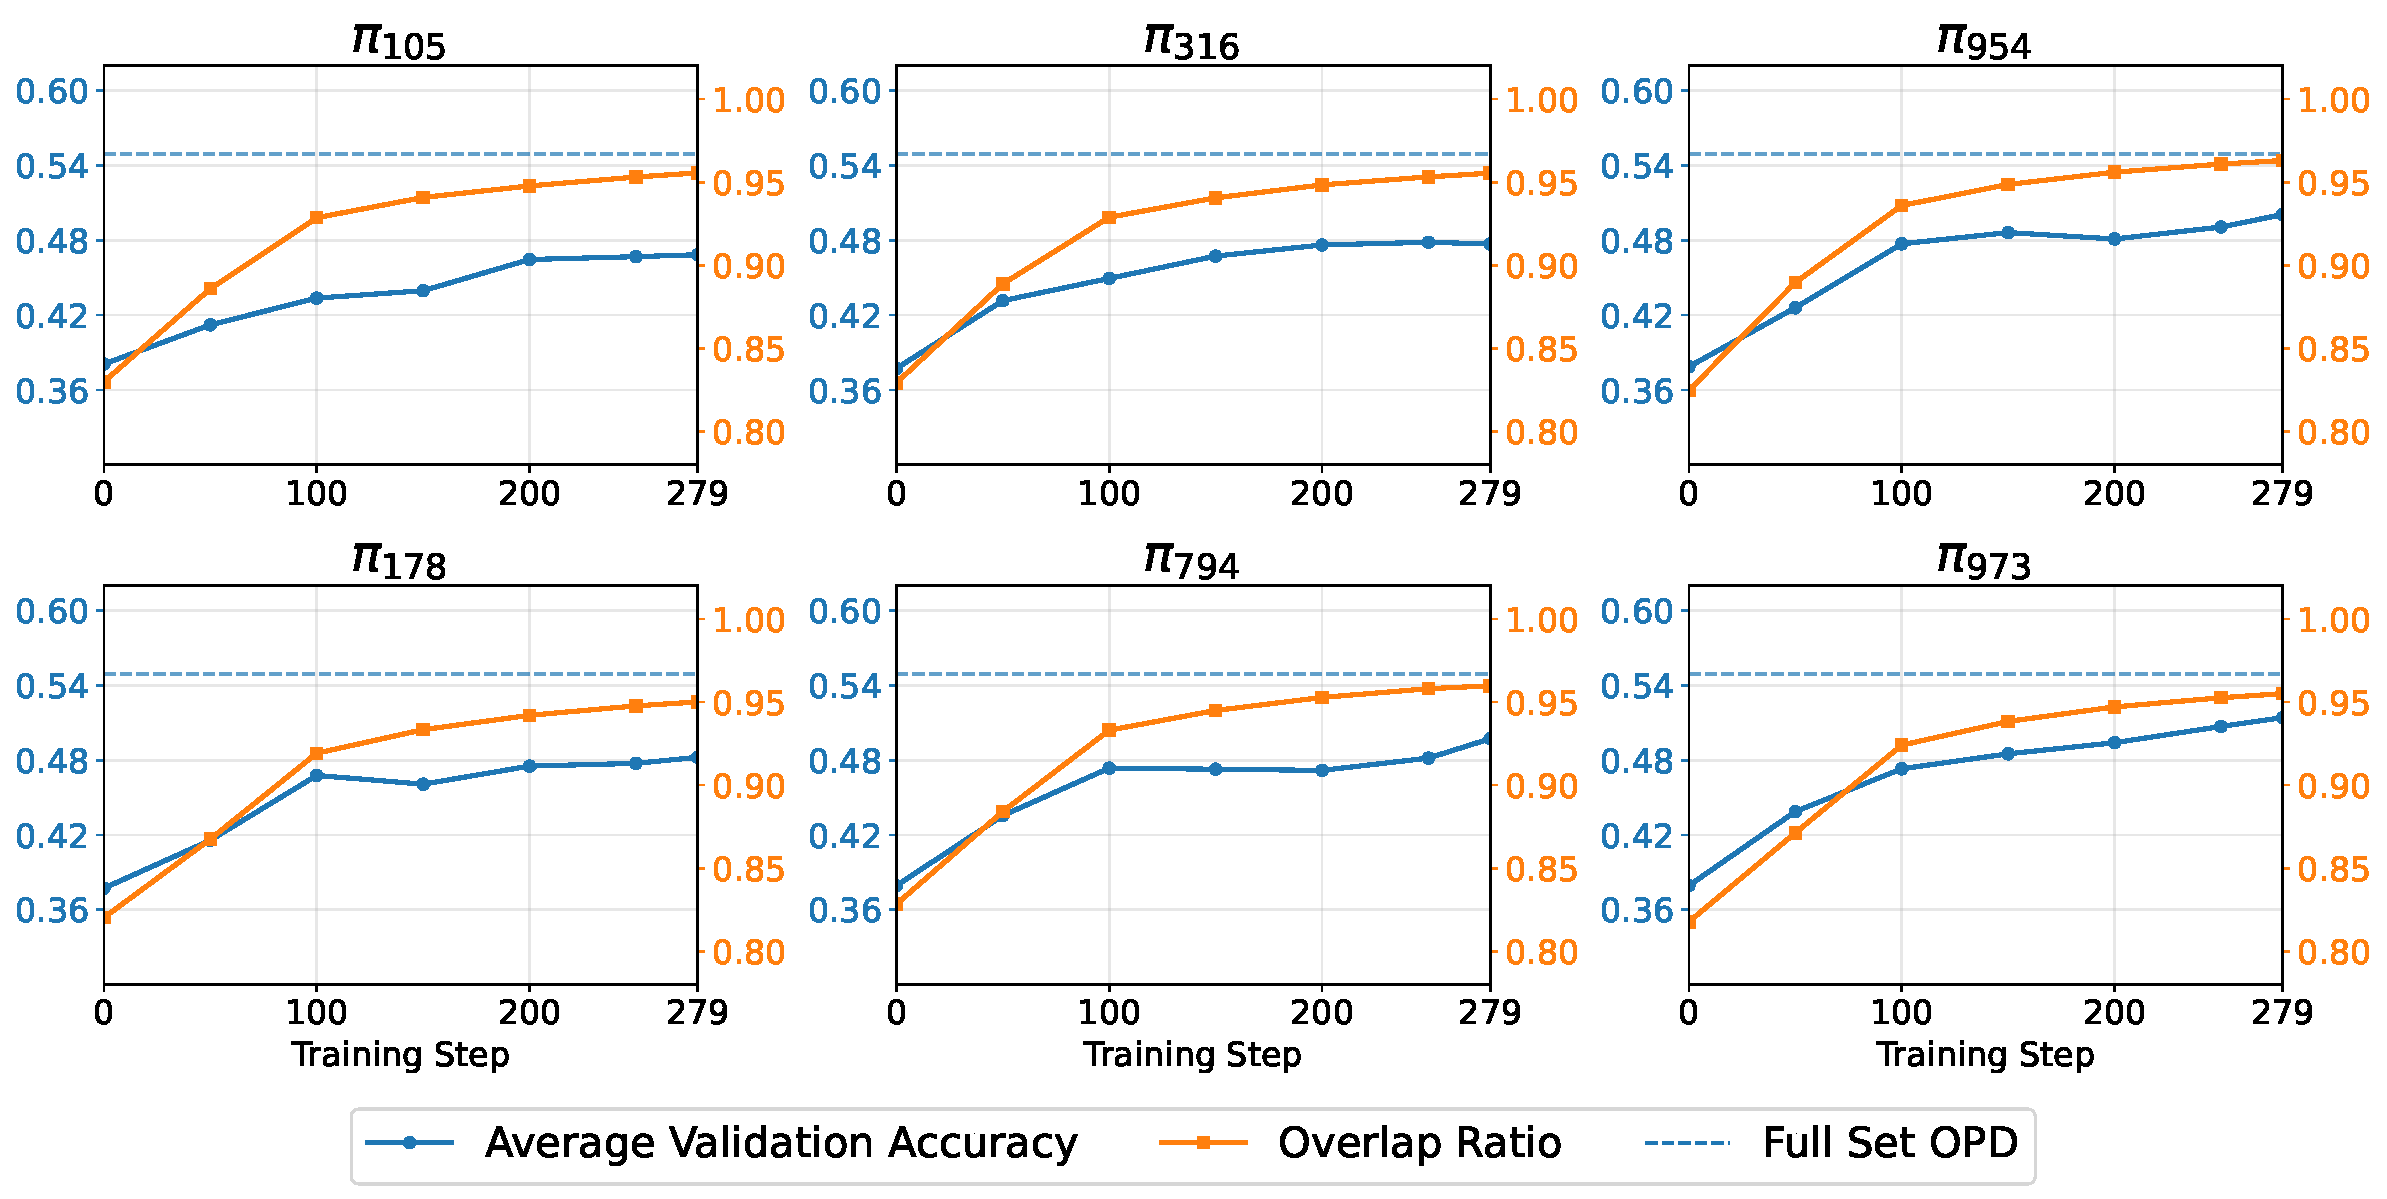
\includegraphics[width=\textwidth]{./images/training.pdf}
    \caption{\textbf{Learning Dynamics of 1-shot OPD.} We visualize the training trajectories of six representative examples across three difficulty levels: two easy problems ($\{\pi_{105}\}$ and $\{\pi_{178}\}$, left), two medium problems ($\{\pi_{316}\}$ and $\{\pi_{794}\}$, middle), and two hard problems ($\{\pi_{954}\}$ and $\{\pi_{973}\}$, right). The solid blue curves denote the Average Validation Accuracy (computed across AMC 2023, AIME 2024, and AIME 2025). The solid orange curves with markers track the Overlap Ratio, indicating progressive token-level policy alignment with the teacher model. The horizontal dashed lines represent the full-set baseline (Full-Set OPD) for comparison. }
    \label{fig:training_curves}
\end{figure*}

\subsection{1-Shot OPD is Effective for Many Examples}
\label{subsubsec:one_shot_effectiveness}

\begin{figure}[htbp]
    \centering
    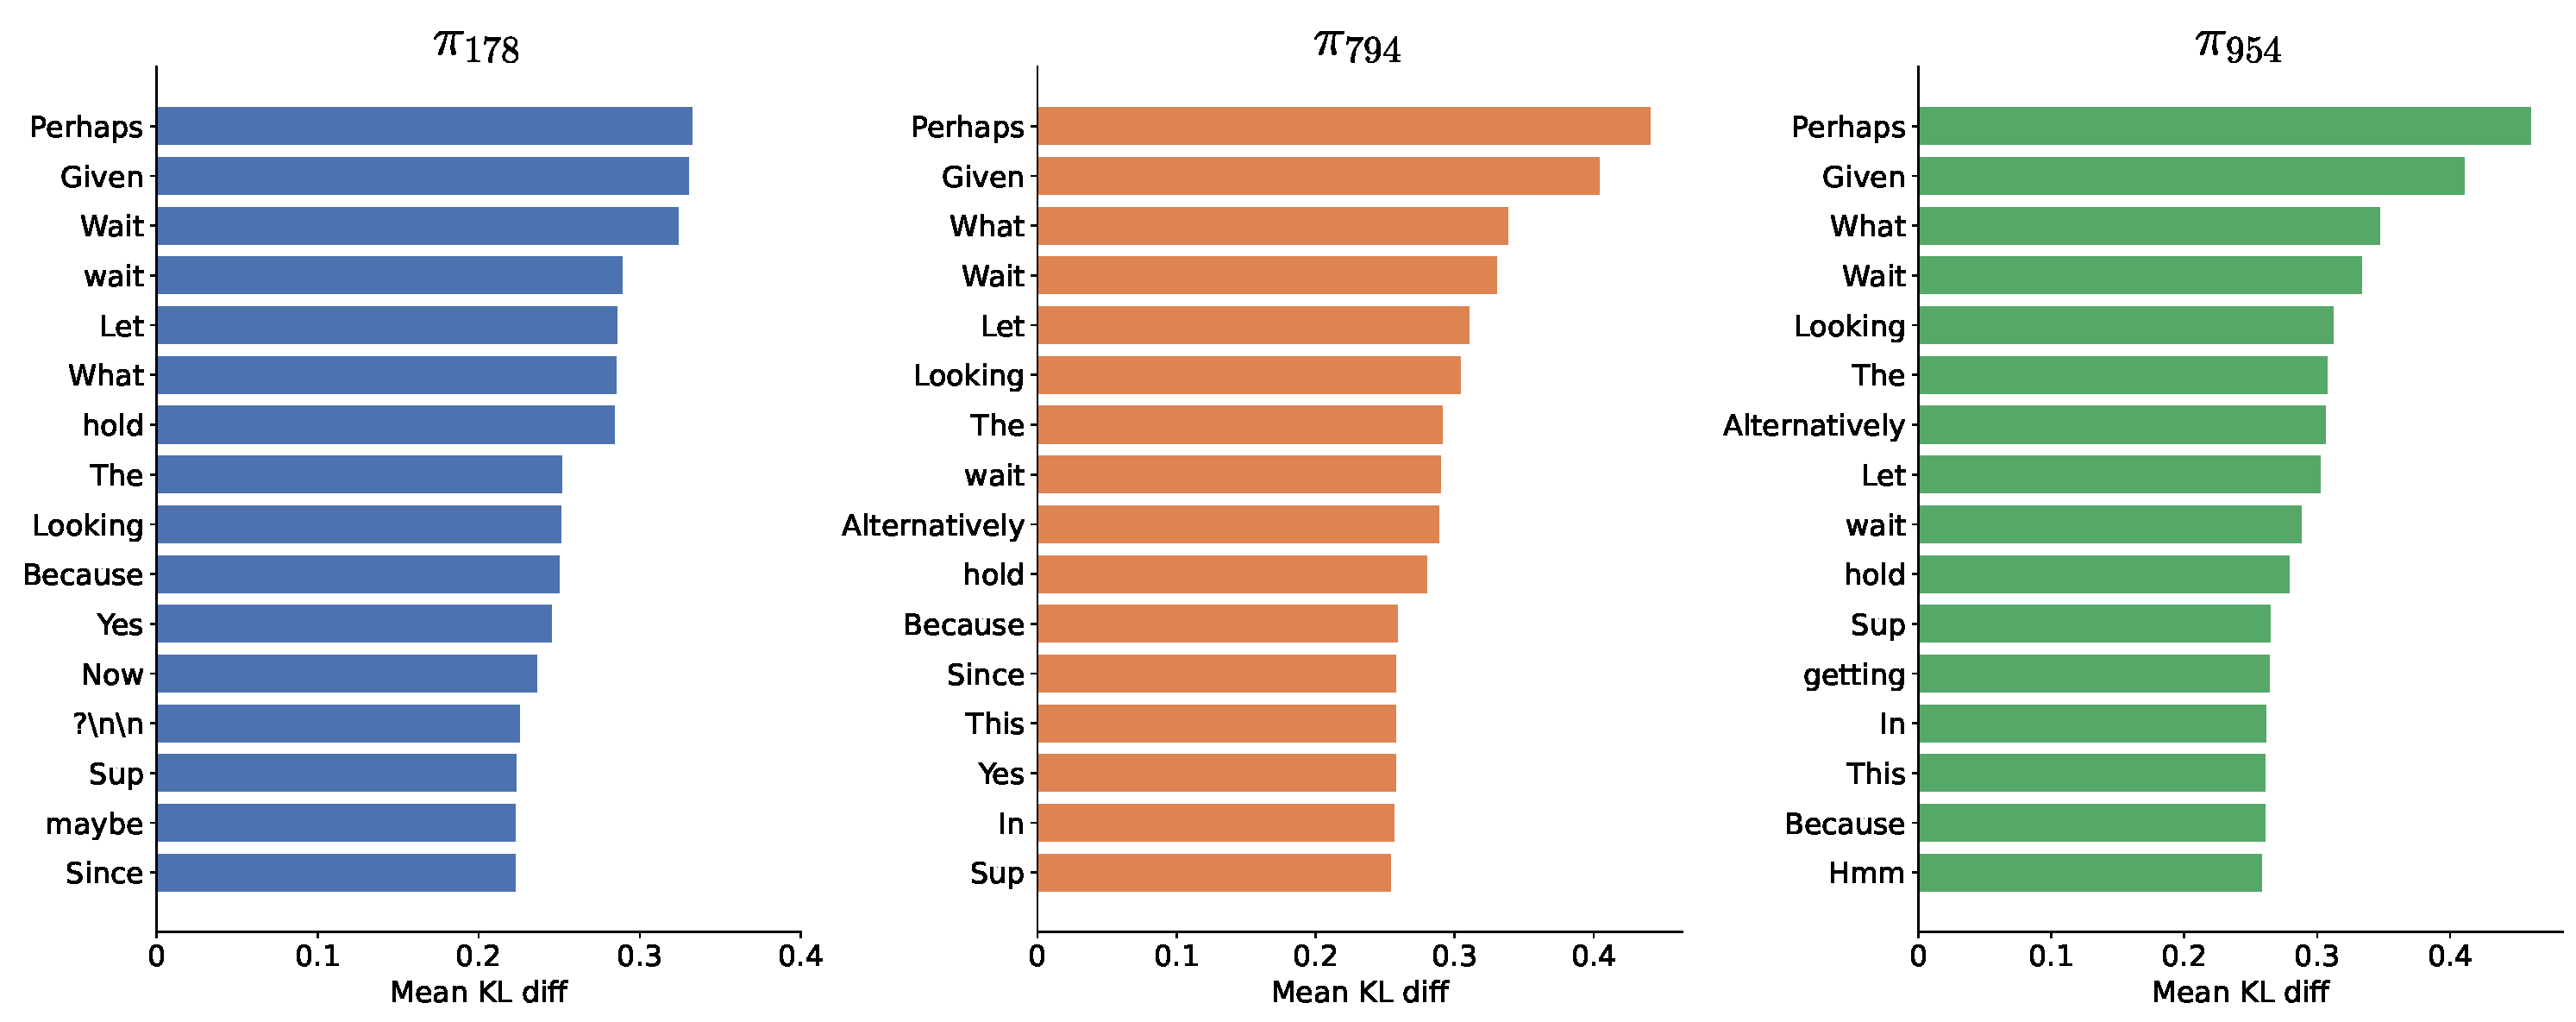
\includegraphics[width=\textwidth]{./images/kl.pdf}
    \caption{\textbf{Per-Token KL Divergence Reduction post 1-Shot OPD.} We report the top 16 tokens with the highest expected KL reduction after distillation for models trained respectively on $\{\pi_{178}\}$ (left), $\{\pi_{794}\}$ (middle), and $\{\pi_{954}\}$ (right).}
    \label{fig:token_kl_reduction}
\end{figure}


First, we randomly sample 8 training examples from each of the Easy, Medium, and Hard categories and train on them individually. The specific indices of sampled examples are listed in Table \ref{tab:opd_accuracies}. During training, we utilize AMC 2023, AIME 2024, and AIME 2025 as the validation set to monitor performance changes over steps. Consistent with our evaluation, we sample 16 solutions per problem with a temperature of 0.7 and a maximum response length of 16,384 tokens, reporting the average accuracy over the 16 samples as our validation metric. Additionally, we track the overlap ratio \citep{li2026rethinking} to measure policy alignment between the student and the teacher. Specifically, we randomly select 100 examples from the DAPO-Math-17K as a held-out set. At each training checkpoint, we perform 16 independent rollouts for each example. Then we report the average proportion of tokens that appear simultaneously in the top-16 vocabulary distributions of both the student and the teacher as the overlap ratio.

We present the evaluation results across benchmarks in Table \ref{tab:one_shot_benchmark_performance}. Moreover, we select some examples to visualize their training trajectories in Figure~\ref{fig:training_curves}. As illustrated in Figure~\ref{fig:training_curves}, the overlap ratio continuously increases, indicating that the student model is progressively aligning with the teacher model. Moreover, the performance improvement demonstrates the effectiveness of 1-shot OPD. We further perform a prolonged training run of 2,000 steps to observe whether 1-shot OPD suffers from overfitting. As shown in Figure \ref{fig:long_training}, the validation performance plateaus after 300 steps and remains stable up to 2,000 steps without any performance decay or policy collapse.


To understand why 1-shot OPD is so effective, we analyze which tokens shift closest to the teacher after distillation. Specifically, we use the held-out set (100 problems) to generate 16 rollouts per problem. Then we compute the reduction in token-level KL divergence between the student and teacher distributions post-distillation and average this KL reduction over all token IDs. For statistical significance, we discard the rare tokens with an overall occurrence frequency of less than 0.01\%. In Figure \ref{fig:token_kl_reduction}, we report the top 16 tokens with the highest KL reduction for models trained respectively on $\{\pi_{178}\}$, $\{\pi_{794}\}$, and $\{\pi_{954}\}$. The results reveal that the tokens aligning most significantly with the teacher after OPD are predominantly structural reasoning, including reflection (e.g., ``Alternatively''), transitions (e.g., ``Wait'', ``Perhaps''), and deductive reasoning (e.g., ``Because'', ``Since''). This indicates that the student can successfully learn the teacher's reasoning patterns by distilling on only a single training example.



\begin{table}[ht!]
\centering
\caption{\textbf{1-Shot OPD Performance Across Mathematical Reasoning Benchmarks.} We compare the student model DeepSeek-R1-Distill-Qwen-1.5B (Base), the teacher model JustRL-DeepSeek-1.5B (Teacher), and the full-dataset distillation baseline (Full-Set) against our 1-shot OPD models. Notably, 1-shot models trained on hard problems consistently outperform those trained on easy problems, with the best-performing example ($\{\pi_{973}\}$) achieving $51.7\%$ average accuracy, nearly matching the Full-Set baseline ($53.7\%$).}
\label{tab:one_shot_benchmark_performance}
\small
\resizebox{0.8\textwidth}{!}{
\begin{tabular}{lccccccc}
\toprule
\textbf{Model} & \textbf{AIME24} & \textbf{AIME25} & \textbf{AMC23} & \textbf{MATH500} & \textbf{Olympiad} & \textbf{Minerva} & \textbf{Avg} \\
\midrule
Base & 31.7 & 23.0 & 60.7 & 82.6 & 34.1 & 22.4 & 42.4 \\
Teacher & 55.8 & 35.8 & 83.4 & 87.4 & 43.4 & 29.8 & 55.9 \\
Full-Set & 51.9 & 34.0 & 78.9 & 86.7 & 44.3 & 26.6 & 53.7 \\
\midrule
\multicolumn{8}{l}{\textit{Easy Problems}} \\
$\{\pi_{5}\}$ & 39.2 & 28.8 & 69.9 & 85.3 & 39.3 & 25.3 & 48.0 \\
$\{\pi_{20}\}$  & 40.3 & 30.6 & 69.1 & 86.2 & 40.8 & 25.7 & 48.8 \\
$\{\pi_{21}\}$  & 41.8 & 29.0 & 71.1 & 85.9 & 39.7 & 26.2 & 48.9 \\
$\{\pi_{63}\}$  & 42.2 & 30.8 & 71.0 & 86.2 & 39.7 & 25.0 & 49.1 \\
$\{\pi_{84}\}$  & 41.0 & 30.1 & 72.6 & 85.6 & 40.6 & 25.8 & 49.3 \\
$\{\pi_{105}\}$ & 42.5 & 27.7 & 70.3 & 86.0 & 41.1 & 25.0 & 48.8 \\
$\{\pi_{178}\}$ & 41.1 & 30.4 & 71.2 & 86.7 & 40.4 & 25.9 & 49.3 \\
$\{\pi_{192}\}$ & 39.8 & 30.2 & 72.0 & 85.7 & 40.1 & 25.7 & 48.9 \\
\midrule
\multicolumn{8}{l}{\textit{Medium Problems}} \\
$\{\pi_{316}\}$ & 39.8 & 30.0 & 73.3 & 86.4 & 40.6 & 25.7 & 49.3 \\
$\{\pi_{487}\}$ & 41.2 & 29.8 & 72.7 & 85.7 & 40.4 & 25.9 & 49.3 \\
$\{\pi_{530}\}$ & 42.1 & 30.7 & 73.1 & 86.5 & 40.2 & 26.8 & 49.9 \\
$\{\pi_{543}\}$ & 40.4 & 29.4 & 73.0 & 86.4 & 41.3 & 26.9 & 49.6 \\
$\{\pi_{661}\}$ & 43.1 & 31.2 & 73.4 & 86.9 & 41.3 & 26.4 & 50.4 \\
$\{\pi_{763}\}$ & 41.5 & 28.1 & 75.6 & 86.7 & 41.2 & 26.8 & 50.0 \\
$\{\pi_{794}\}$ & 44.2 & 30.8 & 74.2 & 86.5 & 41.6 & 25.7 & 50.5 \\
$\{\pi_{820}\}$ & 41.5 & 29.1 & 73.6 & 84.9 & 40.7 & 25.9 & 49.3 \\
\midrule
\multicolumn{8}{l}{\textit{Hard Problems}} \\
$\{\pi_{874}\}$ & 43.3 & 33.1 & 74.3 & 86.6 & 41.0 & 27.1 & 50.9 \\
$\{\pi_{890}\}$ & 45.2 & 29.6 & 76.0 & 85.6 & 42.4 & 26.5 & 50.9 \\
$\{\pi_{948}\}$ & 45.0 & 29.8 & 75.3 & 86.0 & 41.8 & 27.0 & 50.8 \\
$\{\pi_{954}\}$ & 44.8 & 28.5 & 76.9 & 86.9 & 42.6 & 26.7 & 51.1 \\
$\{\pi_{961}\}$ & 44.4 & 30.6 & 73.2 & 87.2 & 41.4 & 26.7 & 50.6 \\
$\{\pi_{973}\}$ & 47.5 & 31.7 & 75.1 & 87.7 & 41.5 & 26.9 & 51.7 \\
$\{\pi_{987}\}$ & 44.8 & 27.7 & 73.6 & 87.5 & 41.2 & 26.4 & 50.2 \\
$\{\pi_{997}\}$ & 44.0 & 30.2 & 75.8 & 85.6 & 42.1 & 26.8 & 50.8 \\
\bottomrule
\end{tabular}
}
\end{table}
